\documentclass[11]{article}
\usepackage{graphicx}
\graphicspath{{images/}}


\title{CS2002 Practical 4 - \\Stable Circuits}
\date{10/04/2018}
\author{Matriculation Number: 160001362}

\begin{document}
	
	\maketitle
	\newpage
	\tableofcontents
	
	\newpage
	\section{Overview}
	This practical specified the development of a system to simulate digital circuits with feedback (generated from a circuit description language) using appropriate data structures and functions. In addition, the practical specified that the output as well as the truth table of the simulated circuit should be appropriately displayed after having been run with suitable inputs.
	\section{Design and Implementation}
		\subsection{Summary}
			The representation of the circuit in the program is an array list (custom data type) of logical gates which is generated by parsing the user input or input from a file into the program. Each gate points to an output wire, as well as to zero to two input wires. These wires are stored in a linked list (also a custom data type). After the circuit has been generated (provided the input is valid) then the truth table for the circuit is output which to be achieved results in the program evaluating the circuit given the possible inputs to check for stabilisation. After the truth table has been output, the data structures utilised are freed.
		\subsection{Data Structures}
			\begin{itemize}
				\item \textbf{Wire}:
					\begin{itemize}
						\item \textbf{name} - a string to store the name of the wire (used as its identifier).
						\item \textbf{val} - the integer value representing the current state of the wire (either 1 or 0).
						\item \textbf{nextVal} - the integer value representing the next state of the wire when the circuit is evaluated (either 0 or 1).
					\end{itemize}
					
				\item \textbf{Gate} (represents a logic gate in the circuit):
					\begin{itemize}
						\item \textbf{op} - stores a string representing the logical operator of the gate.
						\item \textbf{output} - stores a Wire* pointing to the output wire of the gate.
						\item \textbf{input1} - stores a Wire* pointing to the first input wire of the gate (if none then NULL).
						\item \textbf{input2} - stores a Wire* pointing to the second input wire of the gate (if none then NULL).
					\end{itemize}						
				\item \textbf{LinkedList} (used to store wires):
					\begin{itemize}
						\item \textbf{wire} - a Wire* pointing to the wire stored at that node in the linked list.
						\item \textbf{next} - a LinkedList* pointing to the next node in the list.
					\end{itemize}
				\item \textbf{ArrayList} (used to store the list of logical gates):
					\begin{itemize}
						\item \textbf{gates} - a Gate* (array of type Gate) which stores each gate.
						\item \textbf{size} - stores the current size of the array list (i.e. number of Gate structs in gates).
						\item \textbf{capacity} - stores the number of locations in the gates (size cannot exceed capacity).
					\end{itemize}
			\end{itemize}
		\subsection{Files and Libraries}
				\begin{itemize}
					\item \textbf{circuits.c} - This file contains the main function of the program which coordinates the sequence of operations. This file also contains the functions that directly relate to the creation and manipulation of the wires and gates such as creating wires and gates, generating the circuit, generating inputs to the circuit (by converting decimal numbers to binary) \footnote{https://www.javatpoint.com/c-program-to-convert-decimal-to-binary}, evaluating the circuit and computing the next state, as well as stabilising the circuit. This file is also where the fixed value wires 'one' and 'zero' are declared.
					\item \textbf{io.c} - Handles the input and output of the system. The functions contained within this file include the likes of outputting the truth table of the circuit, tokenizing the file/console input, as well as parsing the file/console input and validating it. Also contained within the file is a constant array of strings which stores all of the valid operators (NOT, AND, OR, NAND, NOR, XOR, EQ and IN).
					\item \textbf{linkedlist.c} - This file contains functions that operate on the linked list of wires in the program. This file is similar to the linkedlist file used in the CardTrick practical, only now the linked list has been adapted to store wires instead of cards and has had some additional functions defined. Functions in this file include those to create new nodes, add nodes to the linked list, get the size of the linked list, check if the linked list contains some value, get a node from the list with some given value, reset all of the values in the list, and finally freeing nodes of the list.
					\item \textbf{arraylist.c} - This file contains functions that operate on the array list storing the gates of the circuit in the program. The functions of this file enable adding gate elements to the array list, expanding the array list if the size reaches the list's capacity, creating and initialising an array list, and freeing the memory used by an array list.
					\item \textbf{circuits.h} - Contains definitions for the maximum number of tokens allowed in the program input, the index of each token (output, operator, input1 and input2) in the list of tokens, the default capacity for an array list, and the additional space to be allocated to an array list if its capacity is reached. The file also contains the definitions of the structs of each data structure (Wire, Gate, LinkedList, and ArrayList) as well as the declaration of the global 'wires' LinkedList and definitions for each function in the program.
					\item \textbf{stdbool.h} - Used for intuitive true/false evaluations of conditions.
					
					\item \textbf{stdlib.h} - Used to set appropriate values to NULL as well as enabling the use of malloc and free.
					
					\item \textbf{stdio.h} - Used for input and output.
					
					\item \textbf{string.h} - Used for the string functions necessary to parse the input tokens in io.c.
					\item \textbf{math.h and \_GNU\_SOURCE} - math.h is required for the pow (power) function used to calculate the number of inputs to each circuit and the maximum number of iterations required to stabilise a circuit (if it can be stabilised). \_GNU\_SOURCE is included as math.h is no longer part of the stdlib according to gcc and so this definition must be included to properly import it as well as adding the -lm flag in the make file.
					
	\end{itemize}
	\section{Testing}
		The following is a sample of output generated from testing the solution with various inputs. The sample also demonstrates the improved input validation when entering gates which was developed to satisfy the suggestion in the specification that more robust validation could be completed as an extension:
			\subsection{Input Validation}
				\begin{figure}[h!]
				
					\caption{Demonstrates an error occurring when attempting to create more than 10 gates due to an issue with resizing the array list.}
					\centering
					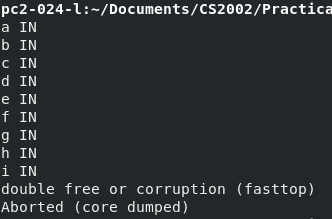
\includegraphics[scale=0.5]{ArrayListResizeError.png}
				\end{figure}
				
				\begin{figure}[h!]
					\caption{Demonstrates inputting more than 10 gates after the array resizing error has been fixed. The bug was fixed by no longer freeing a piece of memory which the array itself need access to.}
					\centering
					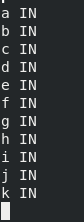
\includegraphics[scale=0.6]{FixedArrayListResize.png}
				\end{figure}
				
				\begin{figure}[h!]
					\caption{Example of dynamic messages being displayed when invalid inputs are entered by robust input validation implemented as an extension.}
					\centering
					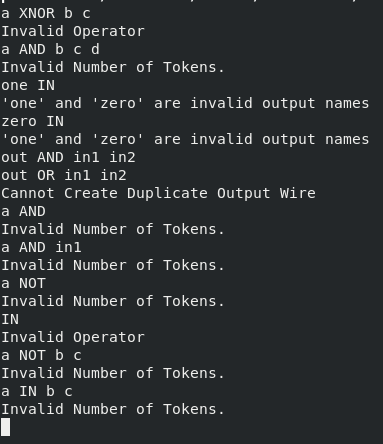
\includegraphics[scale=0.6]{SuccessfulValidation.png}
				\end{figure}
			
			\newpage \clearpage
			\subsection{Generating Output/Truth Tables}
				\begin{figure}[h!]
					\caption{Output of valid circuits being evaluated and truth tables being displayed where appropriate. The output clearly demonstrates that for circuits that do not stabilise, a '?' is displayed, and that for circuits that do stabilise but have no out wire, 0 is displayed. For circuits with an out wire, the values of the out wire are displayed, and for circuits with IN gates, these values are also displayed. The output also demonstrates the use of one of the constant wires (in this case 'one').}				\centering
					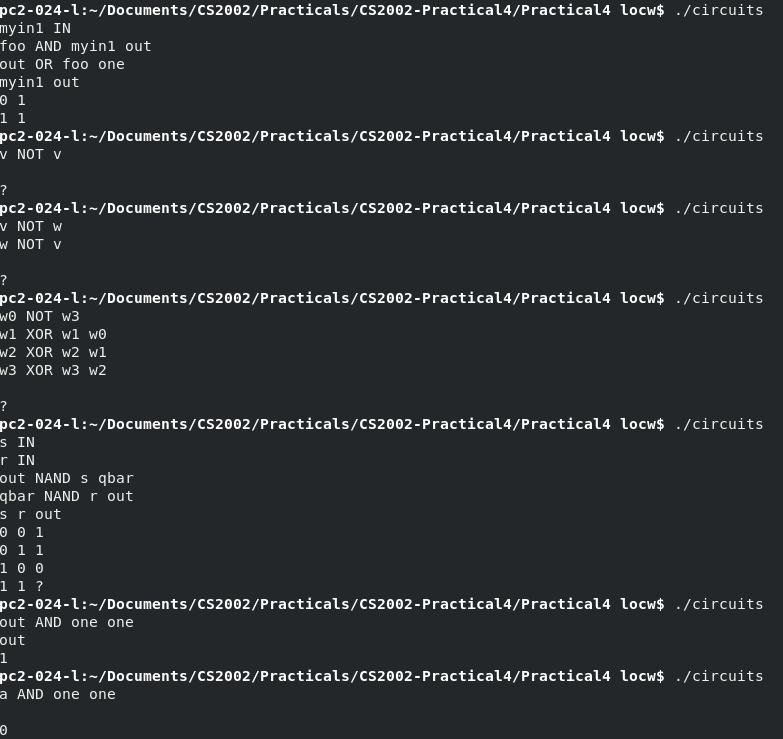
\includegraphics[scale=0.5]{OutputOfValidInput.png}
				\end{figure}
		
	\newpage
	\section{Conclusion and Evaluation}
	In conclusion the requirements specified in the practical document to develop a card trick program have been fully implemented using both an index based implementation as well as non-global pointer based solution utilising a linked list structure. The solutions also both follow the constraints specified in regard to the allowed libraries as well as both only using local instances of data structures. \\\\ To improve upon my solution I would re-implement the way the newColumns struct is initialised in the pointer implementation when the cards are gathered and dealt. The current implementation of the program leaks 1.5MB of memory due to unused allocated memory that was once pointed to by a Columns struct. Without the frees at the end of the main function the program initially had over 3MB of leaked memory. I attempted to free the original columns struct when newColumns is assigned in both the gather and deal functions to reduce the amount from 1.7MB to 0MB however this resulted in a segmentation fault and so I decided to permit some memory not being freed (this would be more of a problem if the trick is repeated many times).
	
				\begin{figure}[h!]
					\caption{Output of 'valgrind ./readmymind'}				\centering
					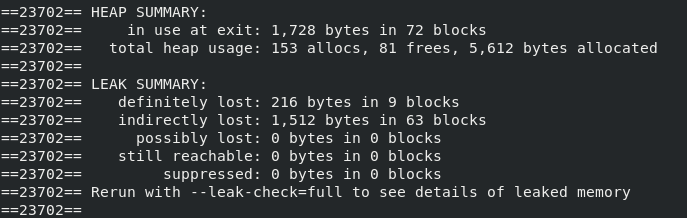
\includegraphics[scale=0.5]{ValGrind.png}
				\end{figure}
	
	
	\section{Extensions}
		\begin{itemize}
			\item \textbf{Improved Input Validation} - 
		\end{itemize}
		
		\begin{figure}[h]
					\caption{Demonstration of repeating trick as well as improved output}				\centering
					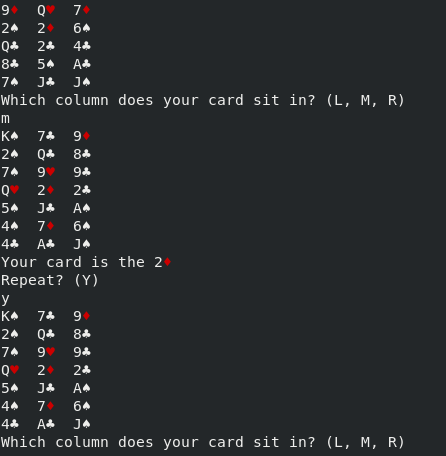
\includegraphics[scale=0.5]{Repeat.png}
		\end{figure}
			
			
		
	\begin{thebibliography}{1}
  		\bibitem{lit1} Mohd Sanad, Zaki Rizvi, \textit{"Singly Linked List Tutorial"}, HackerEarth, https://www.hackerearth.com/practice/data-structures/linked-list/singly-linked-list/tutorial/, (2016).
  	\end{thebibliography}
		
\end{document}